% ----------------------------------------------------------
% Revisão bibliográfica
% ----------------------------------------------------------
\chapter{Revisão da literatura}
\label{chp:revisão}

Os principais aspectos relacionados ao tratamento de evidências para análise forense em nuvem são: coleta, transporte, armazenamento, garantia da cadeia de custódia e reprodutibilidade do processo de coleta. 
%
Este capítulo descreve o estado da arte e discute como a presente proposta se insere nesse contexto.


\section{Soluções para análise forense em nuvem}
\label{sec:estadodaarte}

\marcos{Do jeito que você está apresentando as figuras, você pode ser criticado pelo fato delas terem sempre muito mais informação do que você discute no texto. Não é crítico, mas talvez (se quiser se precaver de críticas) você queira repensar a forma como você discute a solução, para cobrir de forma mais ampla as caixas mostradas na figura (não precisa ser todas as caixinhas, mas pelo menos algumas é bom o leitor saber pra que servem... aí é analisar uma a uma o que potencialmente poderia ser melhor descrito.}

Nesta seção são descritas algumas das principais propostas existentes para coleta de evidências forenses, fornecendo uma visão geral do estado da arte na área.

\subsection{Modelo automático de aquisição de dados para fins forenses}
\label{sec:aquisicaoautomatica}

\marcos{é sempre ``a Figura X'' (maiúsculo, porque é nome próprio), e ``essa figura'' (minúscula, porque não é nome próprio'' - Hamilton : Feito}

O modelo proposto por \cite{ReichertAutoAcquisition:2015}, ilustrado na Figura \ref{fig:ReichertAutoAcquisitionModel}, é um processo de coleta de evidências integrado ao \textit{hypervisor} e disparado por algum sistema de detecção de intrusão. 
%
A partir do momento em que uma ameaça é detectada, o modelo dita que sejam criados instantâneos (\textit{snapshots}) das máquinas virtuais comprometidas. 
%
O intervalo de tempo em que os instantâneos de memória são gerados é configurável, e todos eles são armazenados em persistência.
%
O modelo se preocupa em, de forma automatizada, excluir informações de clientes não relacionados à investigação e também em armazenar o restante em local seguro.
%
O autor não descreve os detalhes do armazenamento, embora afirma que isso deve ser feito de forma ``forensicamente aceitável''.


Para agregar e analisar as evidências coletadas, o modelo faz uso do GRR (\textit{Google Rapid Response} -- Resposta Rápida Google), uma ferramenta de resposta a incidentes criado no projeto 20\% na Google para facilitar análises forenses de forma remota (e.g., acesso de baixo nível ao disco e à memória das máquinas analisadas) \cite{GRRRapidResponse:2013}.
%
O tratamento de evidências usa um motor de regras baseado em um conjunto de descrições de ameaças conhecidas, as quais são armazenadas em um banco de dados.
%
Caso alguma evidência coletada coincida com ameaças armazenadas, esse motor alerta um usuário humano para uma avaliação mais detalhada.
%
Este modelo tem dentre suas principais vantagens a automação do processo de coleta, já que, ao menos em parte, ele dispensa intervenção humana. 

\begin{figure}[htb!]
\footnotesize
\caption{Modelo Automático de Aquisição de Dados Forenses} %\marcos{A fonte do texto está muito pequena... Colocando em 100\% de zoom no pdf, a menor fonte que pode aparecer na figura tem que ser maior ou igual a fonte do footnote do documento. Fontes menores do que isso precisam ser aumentadas. \textbf{Isso vale para todas as figuras.} Além disso: por que ``Actor'' e não ``Ator''...? - Hamilton: Feito}}
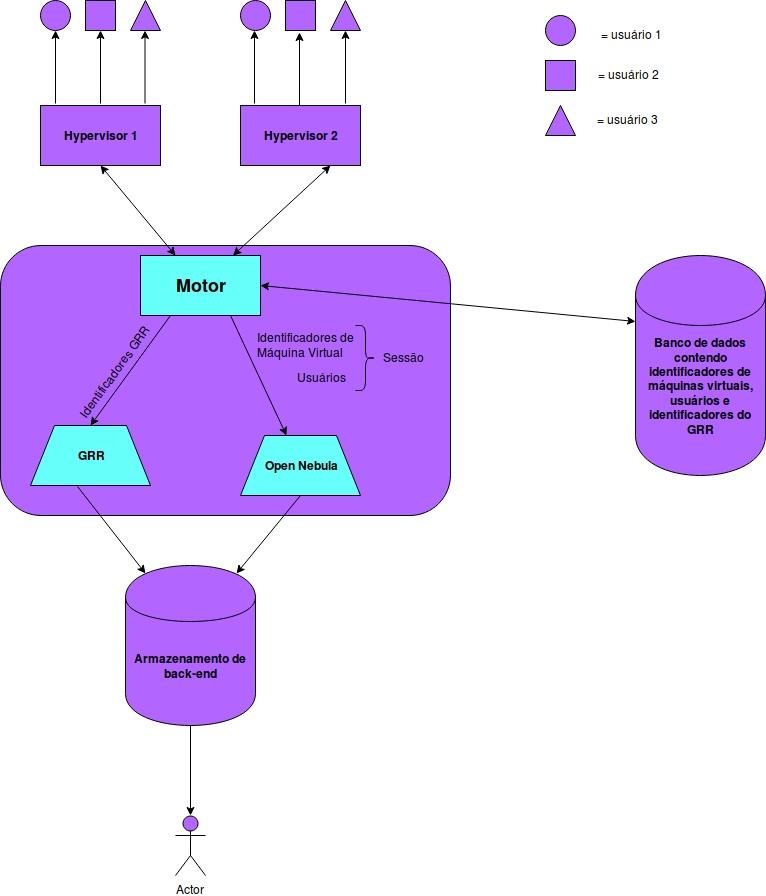
\includegraphics[scale=0.50]{ReichertAutoAcquisitionModel.png}
\centering
\label{fig:ReichertAutoAcquisitionModel}
\begin{center}
Adaptado de \cite{ReichertAutoAcquisition:2015} 
\end{center}
\end{figure}


\subsection{Introspecção em máquina virtual}
\label{sec:VMI}

A proposta de \cite{PoiselVMI:2013} é baseada na técnica de VMI (\textit{Virtual Machine Introspection} -- Introspecção em Máquina Virtual) para coleta de memória volátil. 
%
Essa técnica se apoia no fato de que o o VMM (\textit{Virtual Machine Manager} -- Gerenciador de Máquinas Virtuais) mapeia os recursos alocados para máquinas virtuais nos recursos físicos correspondentes da máquina hospedeira.
%
Este mapeamento é usado para permitir que a memória volátil copiada da máquina virtual seja reconstruída em uma máquina física, para análise posterior.
%
A proposta realiza coleta contínua de instantâneos de memória durante o funcionamento do sistema, sem distinção do que aconteceu antes ou depois do fato de interesse, e todos os instantâneos de memória são armazenados para análise.
%
Visando eliminar a chance de inconsistências no instantâneo de memória volátil, a máquina virtual tem sua execução suspensa durante o processo de extração.


Uma desvantagem da técnica de VMI, mencionada pelo próprio autor \marcos{\cite[Seção {QUAL SECAO?}]{PoiselVMI:2013}} é a necessidade de tradução de endereços de memória da máquina virtual em endereços de memória da máquina física hospedeira.
%
Como essa tradução depende de conhecimento do que está sendo executado na máquina virtual, uma solução baseada em VMI não é completamente portável, sendo necessárias adequações para diferentes clientes.
%
Além disso, o custo computacional dessa tradução é potencialmente elevado \marcos{É isso mesmo? Não ficou claro na frase original o que era ``computacionalmente custoso'', então assumi aqui que é ``a tradução''.}.
%

\subsection{Virtuoso}
\label{sec:virtuoso}

Também na vertente de introspecção de máquina virtual, \cite{Dolan-GavittSemanticGap:2011} propõe o \textit{Virtuoso}, um arcabouço de coleta de informações de processos específicos em uma máquina virtual.
%
O arcabouço funciona em três fases.
%
A primeira realiza um estudo em uma máquina virtual de testes, mapeando o conjunto de instruções executado pelo processo do qual se deseja coletar dados de memória. 
%
A segunda fase traduz o conjunto de instruções mapeados na fase anterior, e então cria um arquivo executável para que o processo seja reproduzido fora da máquina virtual.
%
Para executar as instruções assim extraídas, a terceira fase usa um ambiente na máquina hospedeira capaz de acessar os endereços de memória da máquina virtual, tornando possível coletar instantâneos de memória do processo em execução.
%
A Figura \ref{fig:Dolan-GavittSemanticGap} ilustra o funcionamento desse arcabouço. 


A principal vantagem do Virtuoso é a capacidade de coletar instantâneos de memória de um processo específico.
%
Uma desvantagem importante, entretanto, é que sua atuação se dá apenas após o evento que se deseja avaliar forensicamente.
%


\begin{figure}[htb!]
\footnotesize
\caption{Virtuoso}
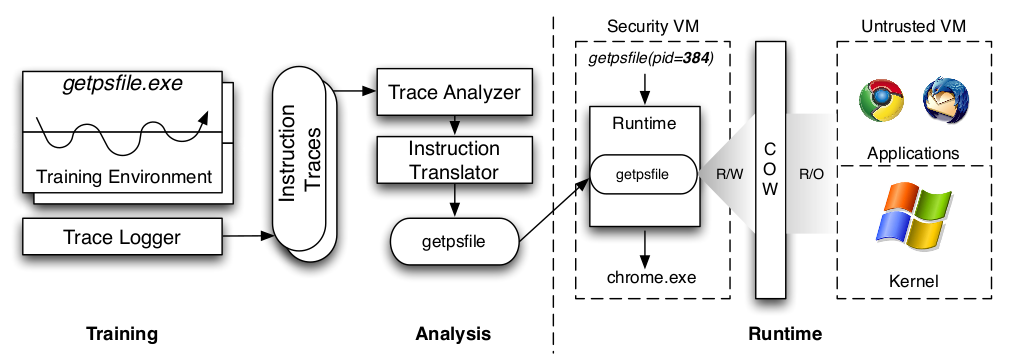
\includegraphics[scale=0.50]{Dolan-GavittSemanticGap.png}
\centering
\label{fig:Dolan-GavittSemanticGap}
\begin{center}
Adaptado de \cite{Dolan-GavittSemanticGap:2011} 
\end{center}
\end{figure}


\subsection{Abordagem baseada em logs}
\label{sec:modelologs}

O arcabouço proposto por \cite{SangLogApproach:2013} é um sistema que funciona em parceria com o provedor de nuvem: o provedor último envia informações ao arcabouço, que por sua vez as armazena em um local adequado, de forma centralizada.
%
O conjunto de informações armazenadas é negociado antecipadamente com o provedor de nuvem, indo desde instantâneos de memória volátil até pacotes trafegados nas interfaces de rede da máquina virtual.
%
O arcabouço coleta informações continuamente e usa cálculo de hash das evidências enviadas pelo provedor de nuvem para garantir que elas não foram alteradas durante o transporte.
%
A Figura \ref{fig:SangLogApproach} ilustra o funcionamento da solução, focando em um caso específico de log de rede, de modo similar ao descrito em \cite{SangLogApproach:2013}.


Assim como as propostas anteriores, o arcabouço em questão também não faz distinção do que aconteceu antes ou depois do fato de interesse, mas  coleta constantemente informações da máquina virtual.
%
Outra potencial limitação é que o arcabouço depende da cooperação do provedor de nuvem. 
%
Tal dependência é uma estratégia considerada fraca pela comunidade forense, pois a prioridade do CSP (\textit{Cloud Service Provider} -- Provedor de Serviços de Nuvem) é a de garantir a disponibilidade do serviço, não de coletar evidências \cite{ClarkeReviewOfChallenges2015}.
%

\begin{figure}[htb!]
\footnotesize
\caption{\textit{A Log Based Approach Model}}
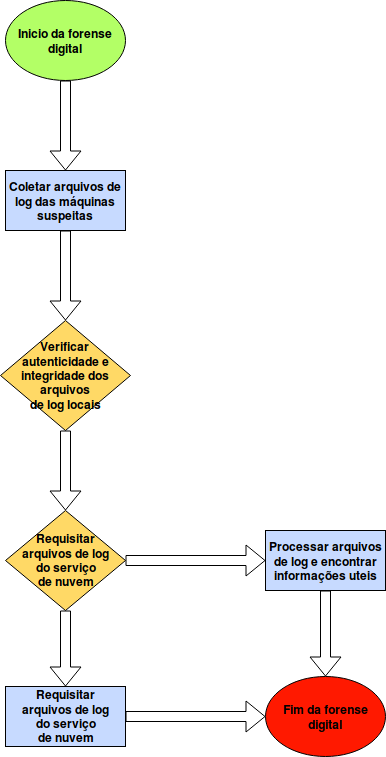
\includegraphics[scale=0.50]{SangLogApproach.png}
\centering
\label{fig:SangLogApproach}
\begin{center}
Adaptado de \cite{SangLogApproach:2013} 
\end{center}
\end{figure}


\subsection{Abordagem baseada em backups}
\label{sec:modelobackup}

O trabalho descrito em \cite{DezfouliBackupApproach:2012} é voltado a dispositivos móveis e tem como principal característica a preocupação com as limitações de armazenamento do dispositivo.
%
Por essa razão, o processo de coleta de instantâneos de memória volátil separa as informações e as armazena por processo ativo \marcos{O que seria ``armazenar por processo ativo''? Eu nem sabia que dava para ``armazenar por processo passivo''...}, de modo a permitir um gerenciamento adequado do espaço em disco ocupado pelas informações. 
%
A solução também se preocupa em descartar informações de processos que foram terminados e removidos da memória, além de buscar u uso consciente do espaço de armazenamento disponível no dispositivo.
%
A Figura \ref{fig:DezfouliBackupApproach} mostra, em alto nível, a forma como o armazenamento de evidências é gerenciado.

Como em diversas outras propostas, processo de coleta de informações de memória volátil em \cite{DezfouliBackupApproach:2012} é executado continuamente, independente de eventos de interesse (e.g., detecção de ameaças).
%


\begin{figure}[htb!]
\footnotesize
\caption{\textit{Backup Approach Model}}
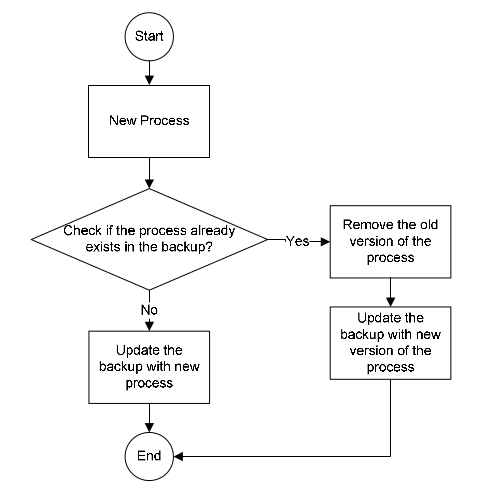
\includegraphics[scale=0.50]{DezfouliBackupApproach.png}
\centering
\label{fig:DezfouliBackupApproach}
\begin{center}
Adaptado de \cite{DezfouliBackupApproach:2012} 
\end{center}
\end{figure}


\subsection{Arcabouço forense para OpenStack}
\label{sec:frost}

A ferramenta FROST (\textit{FoRensic Open Stack Tools} -- Ferramentas Forenses para Arcabouço Open Stack), proposta por \cite{DykstraFROST:2013}, consiste em um conjunto de bibliotecas integradas ao OpenStack, um dos arcabouços de gerenciamento de infra estruturas virtualizadas bastante difundido \cite{StackFramework:2018}.
%
Por meio dessa integração, o FROST expõe um conjunto de APIs que podem ser usadas por aplicações de coleta de evidências forenses.
%
Essas APIs dão acesso a recursos da máquina virtual administrada, tais como disco, logs de tráfego de rede e memória volátil.
%
A proposta descreve apenas o arcabouço, deixando a critério do usuário detalhes como periodicidade e tamanho da coleta, bem como a forma de transporte da evidência e onde ela é armazenada.
%
A Figura \ref{fig:DykstraFROST} ilustra a integração entre FROST e OpenStack.

De todas as propostas avaliadas, a FROST é a única que mostra preocupação com adequação a questões legais e padrões já estabelecidos na indústria forense.
%
Especificamente, o autor declara que FROST segue as práticas definidas no SWGDE (\textit{Scientific Working Group on Digital Evidence} -- Grupo de Pesquisa Scientífica Em Evidência Digital) e do Manual de Busca em Apreensão do Departamento de Justiça Norte-Americano.
%


\begin{figure}[htb!]
\footnotesize
\caption{\textit{FoRensic Open Stack Tools}}
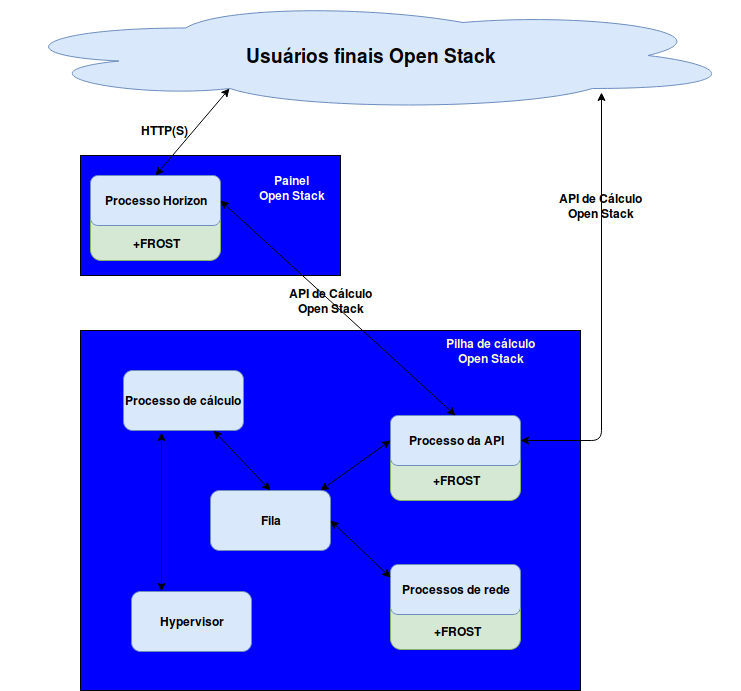
\includegraphics[scale=0.50]{DykstraFROST.png}
\centering
\label{fig:DykstraFROST}
\begin{center}
Adaptado de \cite{DykstraFROST:2013} 
\end{center}
\end{figure}
%


\subsection{Forense como serviço}
\label{sec:frost}

O trabalho descrito em \cite{GeorgeDF2CE:2012} se concentra em monitoramento de rede, operando em uma arquitetura FaaS (\textit{Forense as a Service} -- Forense Como Serviço). 
%
Conforme ilustrado na Figura \ref{fig:GeorgeDF2CE}, a arquitetura da solução consiste em um conjunto de ferramentas com capacidade de descobrir automaticamente as interfaces sob monitoramento, além de coletar evidências de tais máquinas e armazená-las.
%
O processo de auto-descoberta e associação das evidências com usuários de rede é realizado por um motor baseado em ontologias, as quais são armazenadas em um banco de dados próprio.
%
Entretanto, a proposta se concentra apenas no processo de coleta, enquanto a descrição dos mecanismos de armazenamento e transporte não é detalhada.


\begin{figure}[htb!]
\footnotesize
\caption{\textit{Digital Forensic Framework for Cloud Environment}}
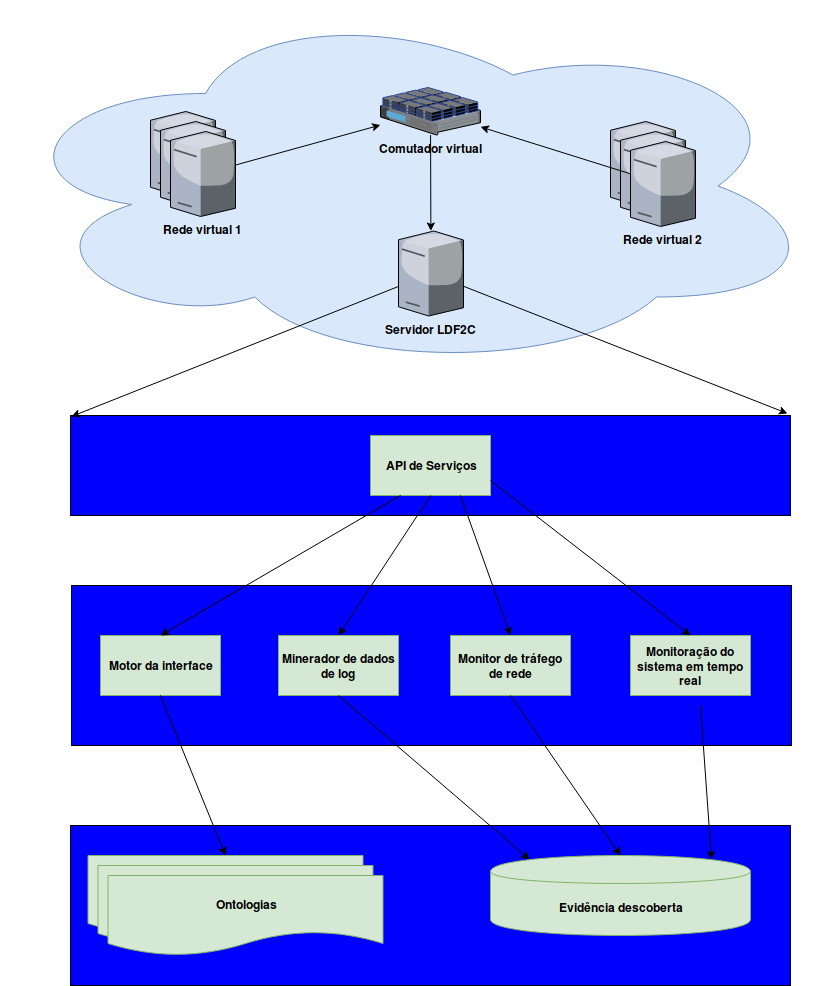
\includegraphics[scale=0.50]{GeorgeDF2CE.png}
\centering
\label{fig:GeorgeDF2CE}
\begin{center}
Adaptado de \cite{GeorgeDF2CE:2012} 
\end{center}
\end{figure}


\subsection{Abordagem de indexação de dados coletados para fins forenses}
\label{sec:indexacaoforense}

Na mesma vertente da solução de forense como serviço descrita na Seção \ref{sec:frost}, \cite{FaaSIndexedSearch:2012} trata o problema de grande volume de dados coletados por meio de um serviço de coleta e indexação de evidências.
%
O serviço espera receber dados da execução do comando unix DD \cite{UnixManPagesDD} nas máquinas alvo, onde, apoiado em processos ETL (\textit{Extract, Transform and Load} -- Extrair, Transformar e Carregar) e MapReduce \cite{WikipediaMapReduce}, os dados são disponibilizados para consulta pelos investigadores.
%
A coleta ocorre continuamente, em intervalos de tempo configuráveis.
%
A Figura \ref{fig:FaaSIndexedSearch} mostra a arquitetura da solução.


Embora interessante, a solução não deixa claro onde os dados são armazenados, nem quem é responsável pela infraestrutura de armazenamento.
%
Também não é discutido como os dados são transportados até o ponto de armazenamento, nem como garantir que esses dados não sejam alteramos no processo.
%


\begin{figure}[htb!]
\footnotesize
\caption{\textit{Digital Forensic as a Service - Indexed Data}}
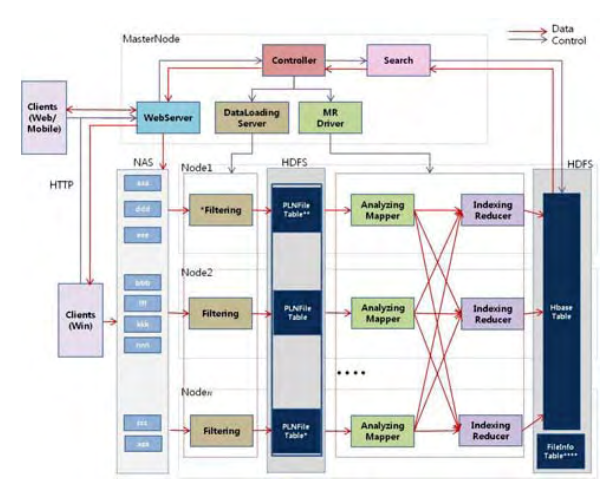
\includegraphics[scale=0.45]{FaaSIndexedSearch.png}
\centering
\label{fig:FaaSIndexedSearch}
\begin{center}
Adaptado de \cite{FaaSIndexedSearch:2012} 
\end{center}
\end{figure}


\section{Aspectos relacionados a coleta de evidência}
\label{sec:coletadeevidencia}

Para uma discussão mais estruturada, a seguir os trabalhos mencionados na Seção \ref{sec:VMI} são agrupados e avaliados com base nos diferentes aspectos que abordam.

\subsection{Acessar e coletar as informações de memória das máquinas virtuais em nuvem}
\label{sec:coletadeevidencia}

Diversos trabalhos de análise forense na nuvem se concentram na coleta de dados ``após o fato'', ou seja, após a intrusão ser detectada \cite{ReichertAutoAcquisition:2015,PoiselVMI:2013,DykstraFROST:2013,GeorgeDF2CE:2012,SangLogApproach:2013}. 
%
Os processos de coleta descritos nesses trabalhos podem ser iniciados de forma manual ou automaticamente, via integração com um mecanismo de detecção de intrusão. 
%
No caso específico de memória volátil, tal forma de coleta não consegue descrever como era a memória antes da intrusão, pois o processo só é acionado depois da detecção do ataque. 
%
%A capacidade de saber como era a memória antes do fato é descrita por \cite{Case_Memory_Forensics:2014} como necessária para viabilizar a abordagem de coletar o suficiente para realizar a investigação pois permite comparar dois instantâneos de memória e minimizar o volume coletado antes do fato. 
Tal limitação pode trazer prejuízos à investigação, dado que algumas análises dependem exatamente da capacidade de se comparar dois momentos da memória \cite{CaseMemoryForensics:2014}. 
%
Entre os trabalhos estudados, a única proposta encontrada que leva tal necessidade em consideração é \cite{DezfouliBackupApproach:2012}, que propõe que o dado seja armazenado no próprio equipamento sob análise.
%
%Infelizmente, entretanto, essa abordagem não é aplicável ao cenário em nuvem, pois leva a perda de informações importantes caso a máquina virtual seja despejada e seus recursos liberados.
Infelizmente, entretanto, a aplicação de tal abordagem no cenário em nuvem é pouco viável, pois pode levar à perda de informações importantes caso a máquina virtual ou contêiner seja desativada, tendo seus recursos liberados.
%

%Ainda na coleta de informações, os autores \cite{Reichert_Auto_acquisition:2015} e \cite{George_DF2CE:2012} sugerem a abordagem de forense ao vivo onde os dados são constantemente coletados sem distinção do antes ou depois do fato. 
Existem ainda trabalhos voltados à coleta de informações durante a execução do sistema, nos quais os dados são constantemente coletados sem distinção do que aconteceu antes ou depois do fato de interesse.
%
Esse é o caso de trabalhos como \cite{PoiselVMI:2013,DykstraFROST:2013,SangLogApproach:2013,Dolan-GavittSemanticGap:2011}, que adotam a estratégia de isolar e parar a máquina virtual para em seguida realizar o processo de coleta. 
%
%Nas duas estratégias citadas anteriormente, o problema do grande volume de informações coletadas não é abordado pelo autores nem o cenário onde é necessário coletar evidências de uma máquina virtual que já foi despejada do pool e os recursos liberados. 
Embora interessantes, as abordagens descritas nesses trabalhos podem levar a um elevado volume de dados coletados.
%
Além disso, elas não tratam o cenário em que é necessário coletar evidências quando são liberados os recursos virtuais que as contêm.


\subsection{Capacidade de reproduzir o processo e obter os mesmos resultados}
\label{sec:reprodutibilidade}

Se, durante uma análise forense, analistas diferentes obtêm resultados distintos ao executar o mesmo procedimento de coleta, a evidência gerada não tem credibilidade, inviabilizando seu uso em um processo legal. 
%
Por essa razão, a reprodutibilidade do processo de coleta é uma parte importante da geração de evidências para análise forense.
%
Infelizmente, entretanto, nenhuma das propostas encontradas na literatura atualmente permite tal reprodutibilidade em cenários de nuvem, em que máquinas virtuais ou contêineres são desativados e seus recursos físicos liberados.
%
Afinal, todas elas dependem da existência do recurso virtual para a repetição do processo de coleta.

\subsection{Não violar privacidade ou jurisdição das partes não envolvidas na investigação}
\label{sec:legais}

Em um ambiente de nuvem pública, remover o \textit{hardware} para análise posterior pode levar à violação de privacidade de usuários.
%
A razão é que o multi-inquilinato desse cenário faz com que uma mesma máquina física guarde informações de diversos clientes, alguns dos quais podem não estar envolvidos na investigação em curso.
%
Diversos trabalhos na literatura tratam esse problema adequadamente, por meio de duas estratégias principais: a primeira, adotada em \cite{ReichertAutoAcquisition:2015,GeorgeDF2CE:2012,PoiselVMI:2013,DykstraFROST:2013,FaaSIndexedSearch:2012}, consiste em coletar dados pertinentes à investigação e armazená-los fora da nuvem; a segunda, empregada em \cite{SangLogApproach:2013} e que constitui um caso específico de \cite{GeorgeDF2CE:2012}, depende da cooperação do provedor de serviços de nuvem para conseguir as informações necessárias à investigação. 
%
Depender do provedor de serviços de nuvem é uma estratégia pouco recomendada, entretanto, pois (1) o volume de dados de usuários pode forçar os provedores a limitar o tamanho dos \textit{logs} armazenados, e (2) caso ocorra uma indisponibilidade causada por um ataque, o objetivo do provedor será o de restabelecer o serviço, não necessariamente o de preservar evidências \cite{ClarkeReviewOfChallenges2015}. 


\subsection{Garantir a cadeia de custódia da evidência}
\label{sec:cadeiadecustodia}

Dentre os trabalhos analisados, apenas \cite{SangLogApproach:2013} aborda a questão da garantia da cadeia de custódia. 
%
Especificamente, o trabalho emprega \textit{hashes} para verificar a integridade da evidência, permitindo a detecção de alterações.
%
Uma limitação desse trabalho, entretanto, é que ele não deixa explícitos os mecanismos que poderiam ser utilizados para impedir acesso não autorizado (e, assim, potencial alteração) aos próprios hashes. 
%
As propostas dos outros autores concentram-se apenas no aspecto técnico da coleta, sem discutir detalhadamente garantia de custódia.
%
Em geral, os trabalhos apenas mencionam que as evidências devem ser coletadas de forma forensicamente aceitável.

\section{Resumo}
\label{sec:resumo}

A Tabela \ref{tab:related-work} mostra um comparativo das soluções estudadas, considerando os aspectos discutidos nesta seção, posicionando as contribuições da proposta apresentada neste trabalho.

\begin{table}[htb!]
\footnotesize
\renewcommand{\arraystretch}{1.4}
\renewcommand{\tabcolsep}{0.5mm}
\centering
\caption{Comparativo de soluções de coleta de informações de memória de máquinas em nuvem para análise forense}
\label{tab:related-work}
\begin{tabular}{p{5.3cm}|L|L|L|L|L|L|L|L|L|}
\textbf{}						& \rot{\fancyname~(esta proposta)} 			& \rot{\cite{GeorgeDF2CE:2012}} 
							& \rot{\cite{PoiselVMI:2013}} 				& \rot{\cite{DykstraFROST:2013}}
							& \rot{\cite{FaaSIndexedSearch:2012}} 			& \rot{\cite{ReichertAutoAcquisition:2015}}	
							& \rot{\cite{SangLogApproach:2013}} 			& \rot{\cite{Dolan-GavittSemanticGap:2011}} 
							& \rot{\cite{DezfouliBackupApproach:2012}} 				
\\ \hline
\textbf{Coleta é contínua?}				& \cfig	& \xfig & \xfig & \xfig & \cfig & \xfig & \cfig & \xfig & \cfig  \\
\textbf{Reproduz o processo sem a VM?} 			& \cfig	& \xfig & \xfig & \xfig & \xfig & \xfig & \xfig & \xfig & \xfig  \\
\textbf{Garante cadeia de custódia?}			& \cfig	& \xfig & \xfig & \xfig & \xfig & \cfig & \cfig & \xfig & \xfig  \\
\textbf{Preserva jurisdição e privacidade?} 		& \cfig	& \cfig	& \cfig	& \cfig	& \cfig	& \cfig	& \cfig	& \cfig	& \cfig	 \\
\end{tabular}
\end{table}
